
\documentclass{beamer}
\usetheme{Zurich}
\usepackage{amsmath, amsfonts, graphicx}
\title{Support Vector Machines}
\author{Charlotte Wickham}
\date{\today}

\begin{document}

\frame{\titlepage}

\section[Outline]{ 	}
\frame{\tableofcontents}

\section{Hyperplane classifiers}


\begin{frame}
	\frametitle{Basic Set Up}
	We have some labeled data from two classes,
	\[
	E = \{(x_1,y_1), (x_2, y_2), \ldots, (x_N, y_N) \},
	\]
	where $x_i\in \mathbb{R}^p$ and $y_i \in \{-1,1\}$.

	\\[14pt]
	Our goal is to come up with a function that will classify new unlabeled data into one of the two classes.
\end{frame}

\begin{frame}
	\frametitle{Separating Hyperplanes}
	Imagine two linearly separable classes.  There are many possible hyperplanes that will separate the groups.
	
	Can define a hyperplane by: 
	\[
	\{x: f(x) = \beta_0 + \beta^Tx = 0\}
	\]
	\begin{itemize}
		\item If we can find $\beta_0$ and $\beta$ for such a separating hyperplane then we can classify a new point, $x'$, by $\text{sign}(f(x'))$.
		\item For linearly separable classes there are many possible separating hyperplanes. How can we choose one?
	 \end{itemize}
\end{frame}

\begin{frame}
	\frametitle{Optimal Separating Hyperplane}
	\begin{itemize}
	\item Choose an optimal criterion for a hyperplane
	\item Maximise the minimal distance from any point to the boundary
	\item Maximise the margin
	\item Can show:
	The distance from any point, $x$, to the hyperplane is proportional to $f(x)$ (equal if $||\beta||=1$).
	\item So we can write the problem as
	\begin{equation*}
	\max_{\beta, \beta_0, ||\beta||=1} C \\
	\text{subject to } y_i(x_i^T\beta + \beta_0) \ge C, \quad i = 1,\ldots, N
	\end{equation*}
	\end{itemize}
\end{frame}

\begin{frame}
	\frametitle{Finding the Optimal Separating Hyperplane}
	Using tricks from convex optimization the problem can be rephrased as maximising
	\begin{equation*}
		L_D = \sum_{i=1}^N \alpha_i - \frac{1}{2}\sum_{i=1}^N\sum_{k=1}^N \alpha_i \alpha_k y_i y_k x_i^Tx_k \\
		\text{subject to constraints \quad}
		\alpha_i \ge 0\\
		\beta = \sum_{i=1}^N \alpha_i y_i x_i\\
		0 = \sum_{i=1}^N \alpha_i y_i \\
		\alpha_i(y_i(x_i^T\beta + \beta_0) -1) = 0 \quad \forall i
	\end{equation*}
	\\[14pt]
	So, if $\alpha_i>0$ then $y_i(x_i^T\beta + \beta_0) = 1$, and $x_i$ is called a support vector.
	Also $\beta$ is calculated only using these support vectors.
\end{frame}

\begin{frame}
	\frametitle{Extending the Optimal Separating Hyperplane}
	\begin{itemize}
		\item In real data classes aren't generally separable.
		\item How can we deal with classification error?
		\item How can we have non linear classification boundaries?
		\item The support vector machine deals with both of these problems
	\end{itemize}
	
\end{frame}

\section{Support vector machines}

\begin{frame}
	\frametitle{Support Vector Machines}
	Classification Error
		\begin{itemize}
			\item Relax the constraint to 
			\begin{equation*}
			y_i(x_i^T\beta + \beta_0) \ge C (1- \epsilon_i), \\
			i = 1,\ldots, N, \quad \epsilon_i\ge 0 \quad \sum_{i=1}^N \epsilon_i \le K
			\end{equation*}
			\item Allows points to be on the ``wrong'' side of the margin.
			\item Misclassified if $\epsilon_i > 1$.
			\item Number of training misclassifications bounded by K.
		\end{itemize}
		Now some of the ``support vectors'' on the wrong side of the margin.
		
	
\end{frame}

\begin{frame}
	\frametitle{Support Vector Machines}
	Nonlinear Boundaries
	\begin{itemize}
		\item Project the original data into a higher dimensional space
		\item Hyperplanes in the higher dimensional space will be non linear boundaries in the original space
		\item Seems like it makes it a much harder problem to solve, but it doesn't, why?
	\end{itemize}
\end{frame}


\end{frame}
\begin{frame}
	\frametitle{Non linear boundaries}
	\item Use a mapping $\phi$ to take values in the original space into a higher dimensional space.
	\item Turns out to find our hyperplane we don't need to know $\phi$ but just 
	\[
	k(x,w) = \phi(x)^T\phi(w)
	\]
	the dot product in the higher dimensional space.
	\item k(x,w) is called the kernel function.
	\item Can think of it as a similarity function.
	\item Some examples,
	\begin{itemize}
		\item linear $k(x,w) = x^Tw$
		\item dth degree polynomial $k(x,w)=(1+x^Tw)^d$
		\item Radial basis $k(x,w)=exp(-||x-w||^2 \gamma)$
	\end{itemize}
\end{frame}

\begin{frame}
	\frametitle{In Practice}
	\begin{itemize}
		\item Need to choose parameters
			\begin{itemize}
				\item Kernel Function
				\item Parameters in kernel function
				\item Tuning parameter (how much misclassification are we allowing?)
			\end{itemize}
		\item Use cross validation to help choose.
		\item Number of support vectors can also be used to diagnose over fitting
	\end{itemize}
\end{frame}

\section{Toy Example}


\begin{frame}
\frametitle{Toy Example}
\begin{columns}[c] % the "c" option specifies center vertical alignment 
	\column{.6\textwidth} % column designated by a command
\setkeys{Gin}{width=\textwidth}
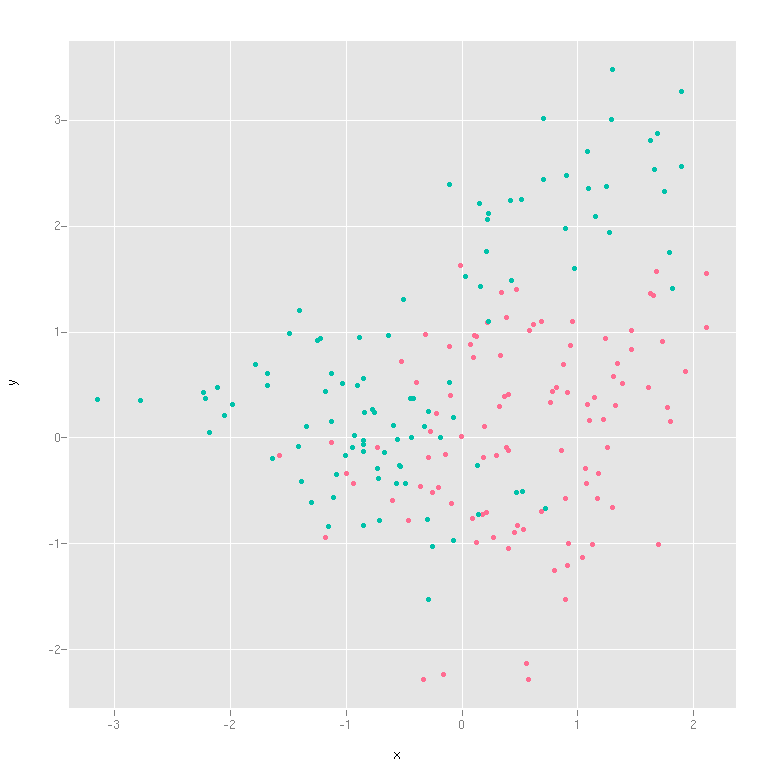
\includegraphics{toyex.png}
	\column{.5\textwidth} 
	\end{columns}
\end{frame}
 
\begin{frame}
\frametitle{Linear Kernels}
\begin{columns}[c] % the "c" option specifies center vertical alignment 
	\column{.5\textwidth} % column designated by a command
		\setkeys{Gin}{width=\textwidth}
		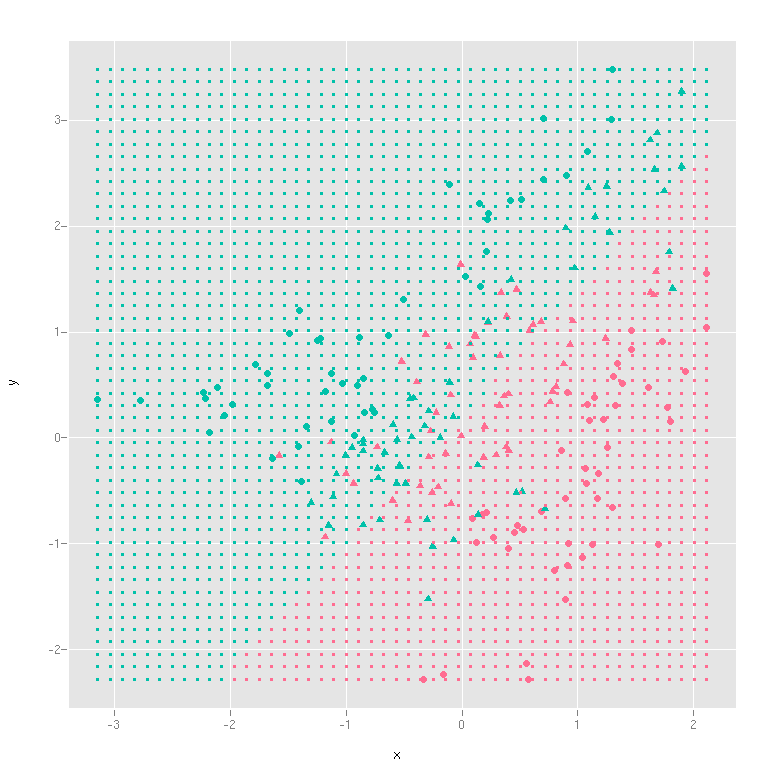
\includegraphics{linc1.png}
		
		Linear kernel C=1

		Number of Support Vectors:  106

		Total Accuracy: 78.5 
	\column{.5\textwidth} 
		\setkeys{Gin}{width=\textwidth}
		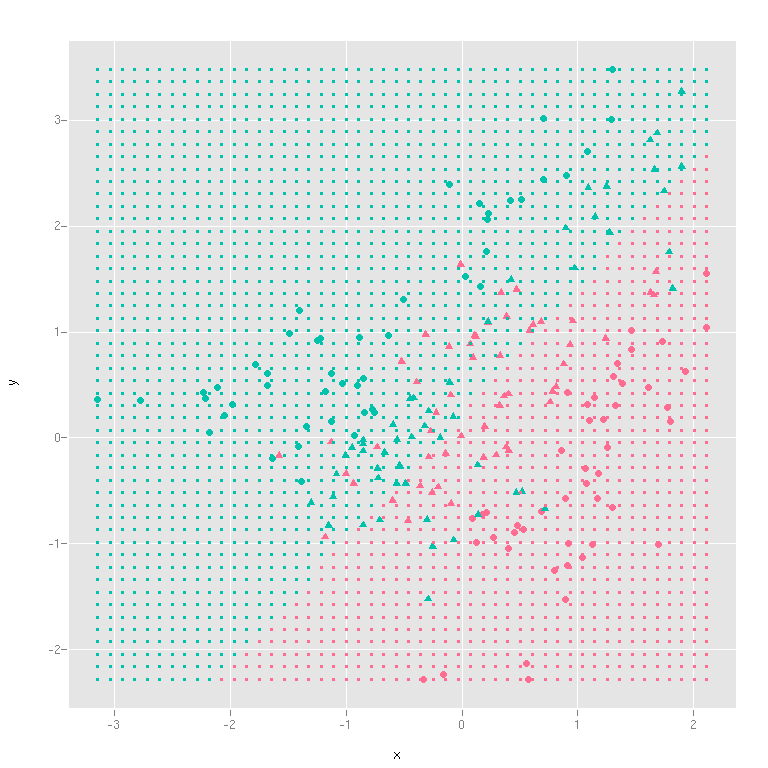
\includegraphics{linc20.png}
		
		Linear kernel C = 20
		
		Number of Support Vectors:  102
		
		Total Accuracy: 78.5 
	\end{columns}
\end{frame}
 

\begin{frame}
\frametitle{RBF Kernels}
\begin{columns}[c] % the "c" option specifies center vertical alignment 
	\column{.5\textwidth} % column designated by a command
		\setkeys{Gin}{width=\textwidth}
		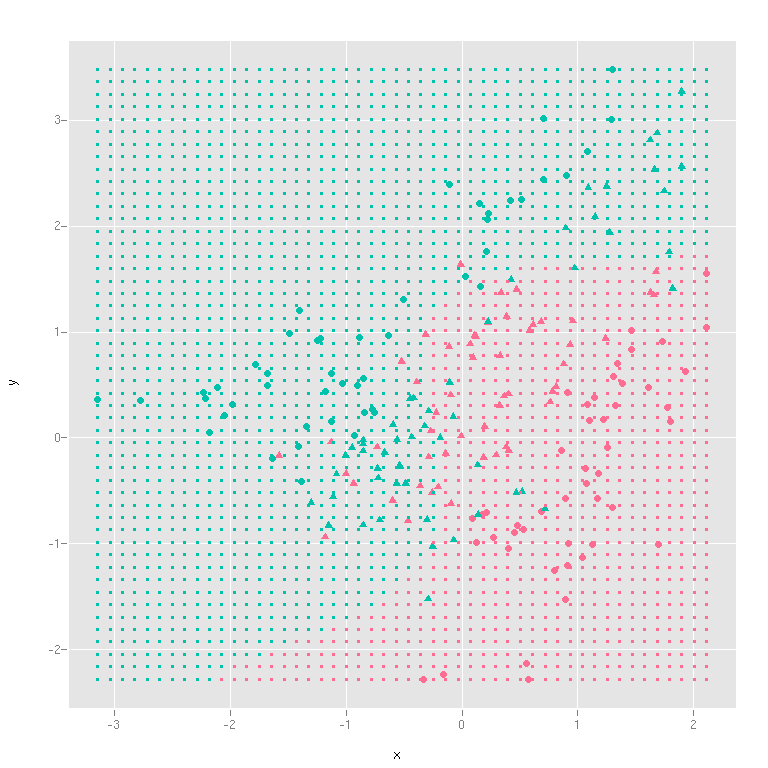
\includegraphics{raddef.png}
		
		Radial kernel C=1, $\gamma = 0.5$

		Number of Support Vectors:  94

		Total Accuracy: 80.5 
	\column{.5\textwidth} 
		\setkeys{Gin}{width=\textwidth}
		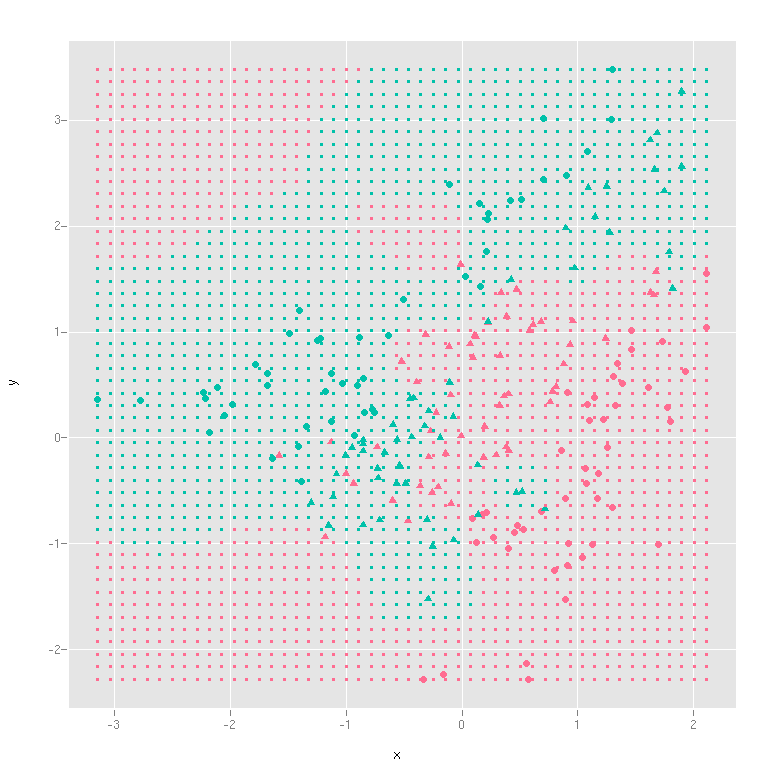
\includegraphics{radbs.png}
		
		Radial kernel C=16, $\gamma = 4$

		Number of Support Vectors:  94

		Total Accuracy: 82.5
	\end{columns}
\end{frame}

\begin{frame}
\frametitle{Polynomial Kernels}
\begin{columns}[c] % the "c" option specifies center vertical alignment 
	\column{.5\textwidth} % column designated by a command
		\setkeys{Gin}{width=\textwidth}
		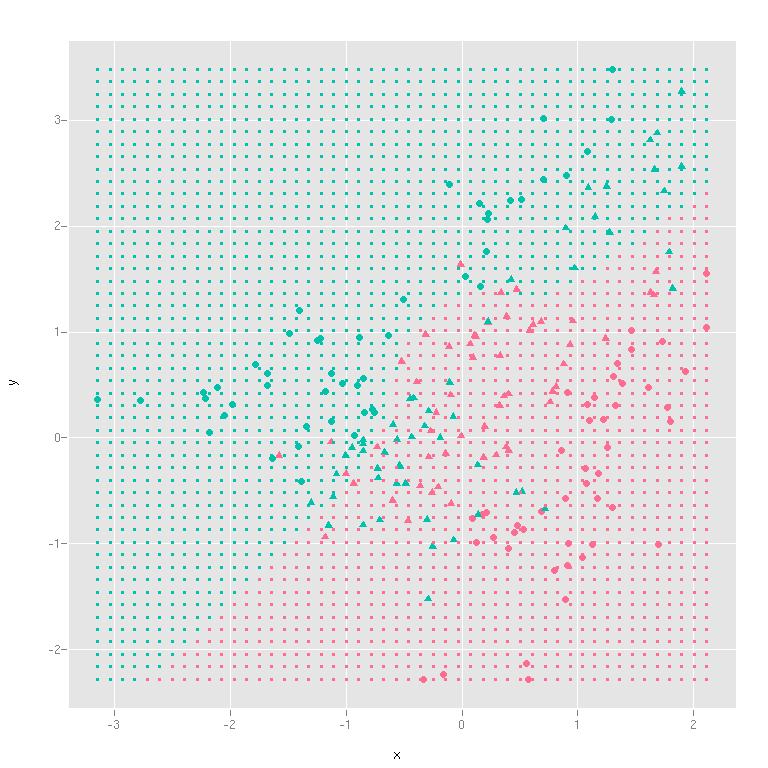
\includegraphics{polydef.png}
		
		Radial kernel C=1, degree = 4

		Number of Support Vectors:  116

		Total Accuracy: 75 
	\column{.5\textwidth} 
		\setkeys{Gin}{width=\textwidth}
		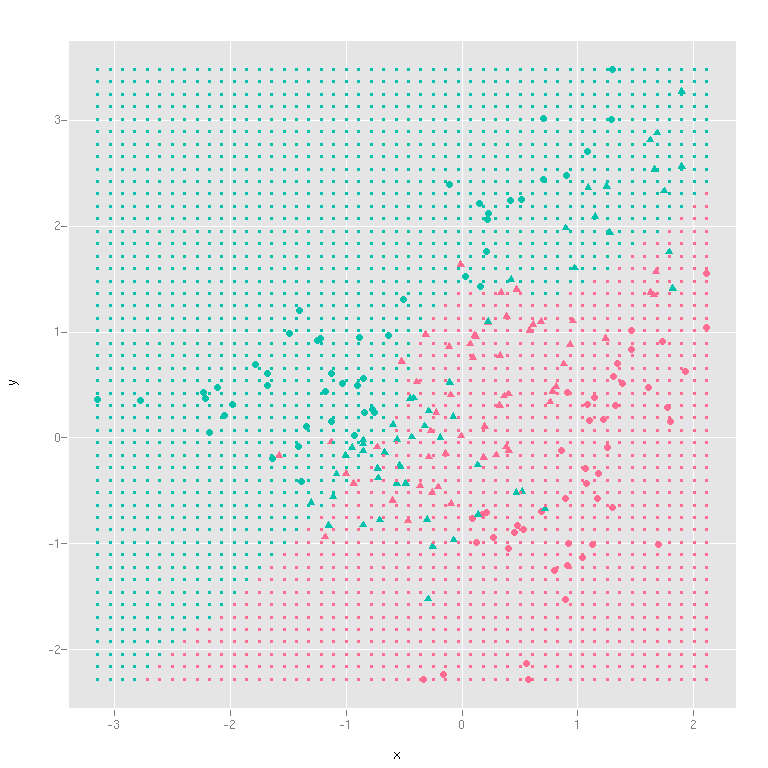
\includegraphics{polyb.png}
		
		Radial kernel C=16, degree = 3

		Number of Support Vectors:  19

		Total Accuracy: 79
	\end{columns}
\end{frame}


\nocite{Hastie:elementsStat:2001}
\nocite{Bishop}
\nocite{chen-tutorial}
\nocite{Hearst}
\nocite{Di}
\nocite{Raquel}
\frame{
\begin{tiny}
\bibliographystyle{plainnat}
\bibliography{refs}
\end{tiny}
}


\begin{frame}
	\frametitle{Computing the support vector classifier}
	Forget mapping into a higher dimension for a moment.\\
	We need to solve the optimization problem
	\begin{equation*}
	\min ||\beta|| \\
	\text{subject to } y_i(x_i^T\beta + \beta_0) \ge 1- \epsilon_i, \quad  \epsilon_i\ge 0 \text{ and } \sum_{i=1}^N \epsilon_i \le constant
	\end{equation*}

	(same as before letting $C = 1/||\beta||$).

	Which is equivalent to solving the following
	\begin{equation*}
	\min_{\beta, \beta_0} \frac{1}{2}||\beta||^2 + \gamma \sum_{i=1}^N \epsilon_i \\
	\text{subject to } y_i(x_i^T\beta + \beta_0) \ge 1- \epsilon_i, \quad  \epsilon_i\ge 0 
	\end{equation*}
	\end{frame}

\begin{frame}
		\frametitle{Computing the support vector classifier...}
		Using tricks from convex optimization this is equivalent to 
		\begin{equation}
		
		\end{equation}
\end{frame}


\end{document}

